\documentclass[12pt,a4paper]{article}

% Packages
\usepackage{amsmath, amssymb}
\usepackage{graphicx}
\usepackage{siunitx} 
\usepackage{caption}
\usepackage{geometry}
\usepackage{url}
\usepackage{cite}
\usepackage{hyperref}
\usepackage{listings}
\usepackage{listings-rust}
\usepackage{xurl}
\usepackage{siunitx}

\lstset{language=Rust, style=boxed}
\geometry{margin=1in}
\graphicspath{{/images}}

\title{Sensors and Actuators for Robotics and
Automation\\Term Project Progress Report III}
\author{Kanisorn Sangchai (ID: 6538020621)}
\date{October 20, 2025}

\begin{document}

\maketitle

\section{Introduction}
This report documents the implementation of Analog-to-Digital Conversion, software configuration, and sensor value read for a thermistor-based temperature sensor system. The STM32H743VIT6 core board by WeAct Studio is used to perform the analog to digital conversion and transmit the measured sensor values via UART communication. The source code for this project can be found in this GitHub repository: \url{https://github.com/Kanisorn-S/sara-project}. The source code for Milestone 2 can be found in the \texttt{Milestone-3} branch: \url{https://github.com/Kanisorn-S/sara-project/tree/Milestone-3}.

\begin{figure}[h]
    \centering
    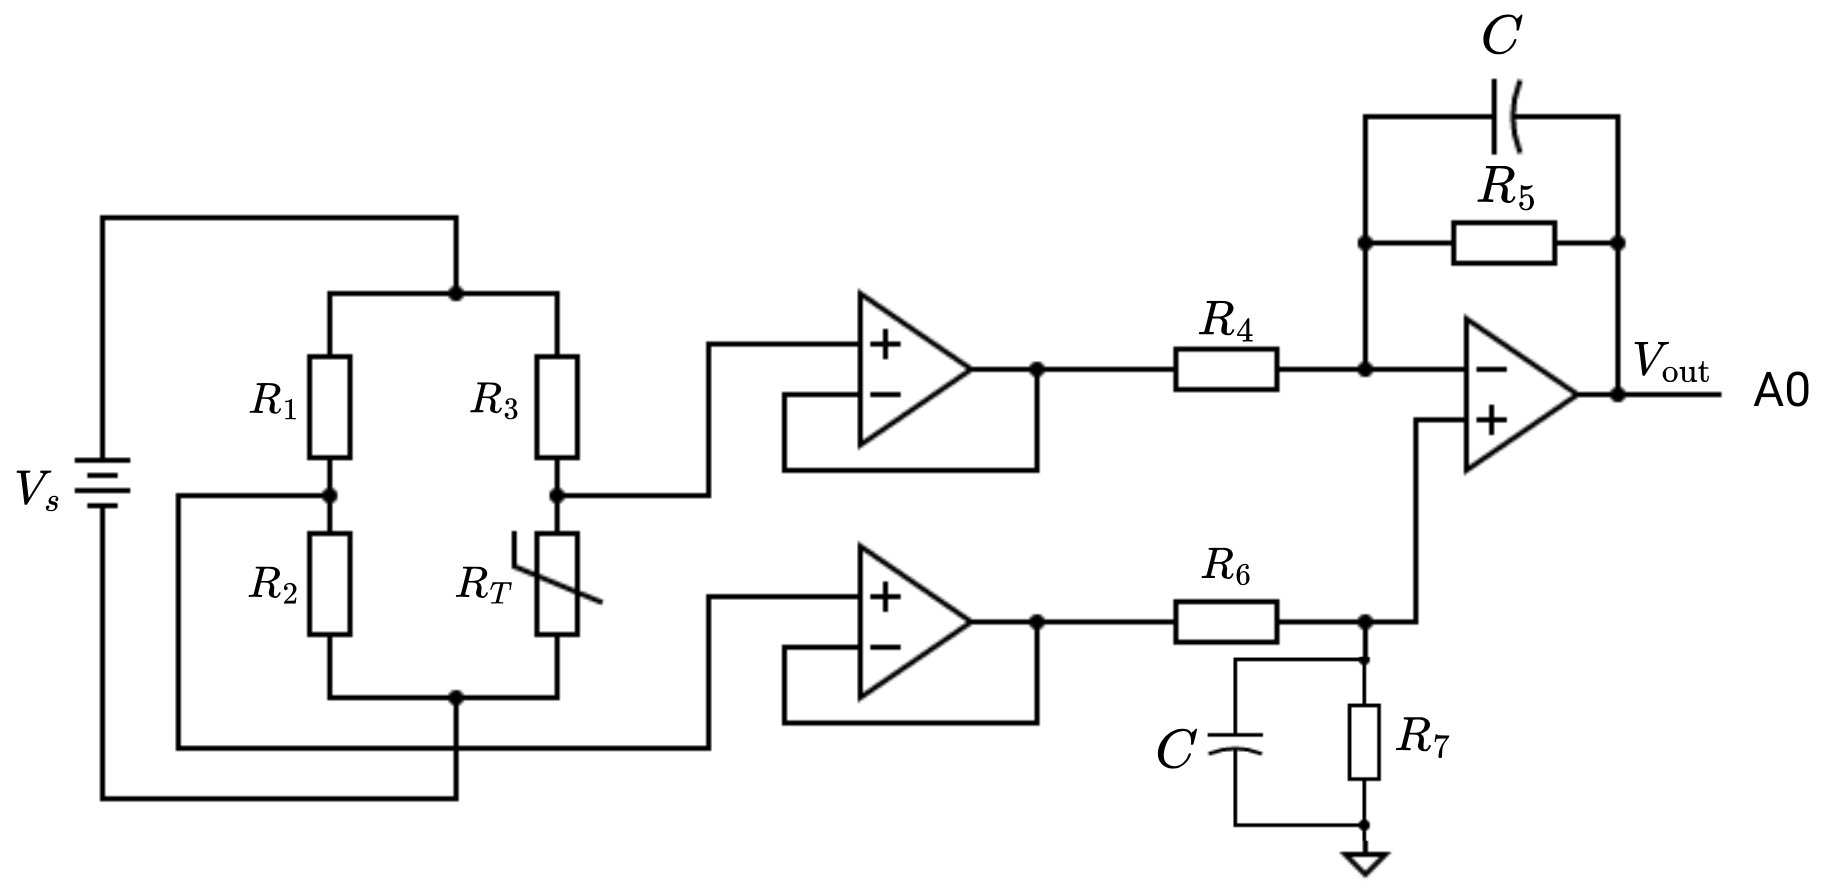
\includegraphics[width=0.9\textwidth]{images/circuit_diagram.png}
    \caption{Original circuit diagram with an adjustable voltage divider added to control the temperature}
    \label{fig:circuit}
\end{figure}

\section{Circuit Design}
An adjustable voltage divider was added to the original circuit design to control the temperature of the thermistor. The voltage divider consists of a potentiometer and a fixed resistor. By adjusting the potentiometer, the voltage across the thermistor can be changed, which in turn changes its temperature.

Figure~\ref{fig:circuit} shows the overall instrumentation circuit consisting of:
\begin{itemize}
    \item A thermistor, which is the transducer of this sensor, in a Wheatstone bridge
    \item 2 Voltage buffers (op-amp in unity gain configuration), one for each bridge output node
    \item An active low-pass filter and differential amplifier for filtering and amplification
\end{itemize}

\subsection{Components}
\subsubsection{Transducer}
For this project, a negative temperature coefficient (NTC) thermistor is used as the transducer. NTC thermistors can be characterised with the B (or $\beta$) parameter equation,

\begin{equation}
    \label{eq:thermistor}
    \frac{1}{T} = \frac{1}{T_0} + \frac{1}{\beta} \cdot \ln{\left(\frac{R_T}{R_0}\right)}
\end{equation}

The selected device is the TTC05103K, which has a nominal (zero-power) resistance of 
\SI{10}{k\ohm} at \SI{25}{\celsius}, a tolerance of $\pm 10\%$, and $\beta=4050 \text{K}$~\cite{thermistor}. 

\subsubsection{Wheatstone Bridge}
A Wheatstone bridge circuit was implemented to measure the resistance of the thermistor.  
Three precision metal film resistors of $10\,\text{k}\Omega \pm 100\,\Omega$~\cite{resistor} were chosen to form the reference arms of the bridge.  
At $25^{\circ}\text{C}$, the thermistor has a nominal resistance of $10\,\text{k}\Omega \pm 1\,\text{k}\Omega$,  
which balances the bridge.  

The bridge is powered with a $3.3\,\text{V}$ supply provided by the STM32H743 core board.  
At balance (25$^{\circ}$C), the differential output voltage of the bridge is close to zero.  

\subsubsection{Voltage Buffer}
Two voltage buffers were implemented using an LM358N operational amplifier. The LM358N is a low-power dual op-amp ~\cite{op-amp}. The buffers were configured in a unity-gain configuration (voltage follower), ensuring that the output voltage directly follows the input from the bridge while providing high input impedance and low output impedance.

\subsubsection{Active Low-pass Filter and Differential Amplifier}
Since temperature changes slowly, high-frequency noise should be filtered out. An active low-pass filter and differential amplifier was implemented using an LM358N operational amplifier.  
The target cutoff frequency was chosen as \SI{5}{Hz} with a voltage gain of 2. The resistance $R_5$, is selected to be $\SI{47}{\kilo\ohm}$. The values for $R_4$ and $C$ were then selected to try and achieve the desired cutoff frequency and voltage gain. The values for $R_6$ and $R_7$ are selected to be the same as $R_4$ and $R_5$ respectively to simplify the transfer function for the differential amplifier.

\textbf{Selected values:}
\begin{itemize}
    \item $R_4 = R_6 = \SI{22}{\kilo\ohm}$
    \item $R_5 = R_7 = \SI{47}{\kilo\ohm}$
    \item $C = \SI{0.47}{\micro\farad}$
\end{itemize}

These values provide a practical cutoff frequency of $\approx \SI{7.2}{Hz}$ and gain of $\approx 2.14$, which are sufficiently close to the design targets. More detailed calculations are provided in Section~\ref{sec:math-model} and~\ref{sec:filter}

\section{Mathematical Model}
\label{sec:math-model}
The Wheatstone bridge output voltage is given by:
\begin{equation}
    \Delta V = V_s \cdot \left( \frac{R_2}{R_1 + R_2} - \frac{R_T}{R_3 + R_T} \right)
    \label{eq:wheatstone}
\end{equation}

With $R_1=R_2=R_3=R_{ref}$, \eqref{eq:wheatstone} simplifies to

\begin{equation}
    \Delta V = V_s \cdot \left(\frac{1}{2} - \frac{R_T}{R_{ref} + R_T} \right)
    \label{eq:simplified-wheatstone}
\end{equation}

We rearrange \eqref{eq:simplified-wheatstone} to solve for $R_T$, we get

\begin{equation}
    R_T = \left(\frac{V_s - 2\Delta V}{V_s + 2\Delta V}\right) \cdot R_{ref}
    \label{eq:rt}
\end{equation}

We substitute \eqref{eq:rt} into \eqref{eq:thermistor}

\begin{equation}
    \label{eq:t-to-v}
    \frac{1}{T} = \frac{1}{T_0} + \frac{1}{\beta} \cdot \ln{\left( \left(\frac{V_s - 2\Delta V}{V_s + 2\Delta V}\right) \cdot \frac{ \cdot R_{ref}}{R_0}\right)}
\end{equation}

The voltage buffer is for preventing current from affecting the measurement; therefore, the equation for the buffer is simply

\begin{equation}
    \label{eq:vbuf-to-deltav}
    V_\text{buffer} = \Delta V
\end{equation}

For the amplifier stage, the equation of a differential amplifier is:

\begin{equation}
    V_\text{out} = \frac{R_5}{R_4} \cdot V_\text{buffer}
    \label{eq:vout-to-vbuffer}
\end{equation}

where the gain is

\begin{equation}
    A_v= \frac{R_5}{R_4}
    \label{eq:gain}
\end{equation}

Firstly, the resistance $R_5$ is selected to be $\SI{47}{\kilo\ohm}\pm\SI{470}{\ohm}$ (MF0W4FF4702P50 from \cite{resistor}).To achieve the desired voltage gain of 2, we solve \eqref{eq:gain} for $R_4$, which we get $R_4\approx\SI{23.5}{\kilo\ohm}$. The closes standard resistance available was $\SI{22}{\kilo\ohm}\pm\SI{220}{\ohm}$ (MF0W4FF2202P50 from \cite{resistor}). We now use this value to calculate the actual voltage gain from \eqref{eq:gain}, which gives us 

\begin{equation*}
    A_v= \frac{R_5}{R_4} = \frac{\SI{47}{\kilo\ohm}}{\SI{22}{\kilo\ohm}} \approx 2.14 
\end{equation*}

Calculating for the error,

\begin{equation*}
    \delta A_v = A_v (\frac{\delta R_4}{R_4} + \frac{\delta R_5}{R_5}) = 2.14 (\frac{\SI{220}{\ohm}}{\SI{22}{\kilo\ohm}} + \frac{\SI{470}{\ohm}}{\SI{47}{\kilo\ohm}}) \approx 0.04
\end{equation*}

$A_v\approx 2.14 \pm 0.04$.

\section{Filtering Analysis}
\label{sec:filter}
The cutoff frequency $f_c$ is determined by:

\begin{equation}
    f_c = \frac{1}{2 \pi R_5 C}
    \label{eq:cutoff}
\end{equation}

Firstly, the resistance $R_5$ is selected to be $\SI{47}{\kilo\ohm}\pm\SI{470}{\ohm}$ (MF0W4FF4702P50 from \cite{resistor}). To achieve the desired cutoff frequency of \SI{5}{Hz}, we solve \eqref{eq:cutoff} for $C$, which we get 

\begin{equation*}
    C = \frac{1}{2 \pi R_5 f_c} = \frac{1}{2 \pi (\SI{47}{\kilo\ohm}) (\SI{5}{Hz})} \approx \SI{0.67}{\micro\farad} 
\end{equation*}

The closest standard capacitance available was $\SI{0.47}{\micro\farad}\pm\SI{47}{\nano\farad}$ (RDER72E474K4K1H03B from \cite{capacitor}).We now use this value to calculate the actual cutoff frequency from \eqref{eq:cutoff}, which gives us 

\begin{equation*}
    f_c = \frac{1}{2 \pi R_5 C} = \frac{1}{2 \pi (\SI{47}{\kilo\ohm}) (\SI{0.47}{\micro\farad})} \approx \SI{7.2}{Hz} 
\end{equation*}

Calculating for the error,

\begin{align*}
    \delta f_c &= f_c (\frac{\delta R_5}{R_5} + \frac{\delta C}{C}) \\
    &= \SI{7.2}{Hz} (\frac{\SI{470}{\ohm}}{\SI{47}{\kilo\ohm}} + \frac{\SI{47}{\nano\farad}}{\SI{0.47}{\micro\farad}}) \approx \SI{0.8}{Hz}
\end{align*}

$f_c\approx\SI{7.2}{Hz}\pm\SI{0.8}{Hz}$

\section{Demonstration and Verification}

To demonstrate and verify the result of the implemented circuit, we compare the temperature measured from our circuit with the temperature measured from a digital thermometer.

\begin{figure}[h]
    \centering
    \includegraphics[width=0.8\textwidth]{images/circuit_measurement.jpg}
    \caption{Voltage reading from the circuit.}
    \label{fig:circuit-measure}
\end{figure}

\begin{figure}[h]
    \centering
    \includegraphics[width=0.8\textwidth]{images/thermometer.jpg}
    \caption{Temperature measured by a digital thermometer.}
    \label{fig:thermometer}
\end{figure}

From Figure~\ref{fig:circuit-measure}, we get that $V_{\text{out}}=\SI{48.4}{\milli\volt}$. Since we measured the voltage using the Sanwa CD770 Digital Multimeter, which has an accuracy when reading DC Voltage below \SI{400}{\milli\volt} of $\pm (0.5 \% \text{rdg} + 2 \text{dgt})$~\cite{multimeter}, the value for $V_{\text{out}}$ is $\SI{48.4}{\milli\volt} \pm \SI{0.4}{\milli\volt}$. We substitute $V_{\text{out}}$ into \eqref{eq:vout-to-vbuffer} to solve for $V_{\text{buffer}}$

\begin{equation*}
    V_{\text{buffer}} =  \frac{R_4}{R_5} \cdot V_{\text{out}}
    =  \frac{\SI{22}{\kilo\ohm}}{\SI{47}{\kilo\ohm}} \cdot \SI{48.4}{\milli\volt} \approx \SI{22.6}{\milli\volt}
\end{equation*}

Calculating for the error,

\begin{align*}
    \delta V_{\text{buffer}} 
    &= V_{\text{buffer}} (\frac{\delta R_4}{R_4} + \frac{\delta R_4}{R_4} + \frac{\delta V_{\text{out}}}{V_{\text{out}}}) \\
    &= \SI{22.6}{\milli\volt} (\frac{\SI{220}{\ohm}}{\SI{22}{\kilo\ohm}} + \frac{\SI{470}{\ohm}}{\SI{47}{\kilo\ohm}} + \frac{\SI{0.4}{\milli\volt}}{\SI{48.4}{\milli\volt}}) \approx \SI{0.6}{\milli\volt}
\end{align*}

From \eqref{eq:vbuf-to-deltav}, we get

\begin{equation*}
    \Delta V = \SI{22.6}{\milli\volt} \pm \SI{0.6}{\milli\volt}
\end{equation*}

We now substitue $\Delta V$ into \eqref{eq:t-to-v} and solve for the temperature $T$

\begin{align*}
    T &= \left(\frac{1}{T_0} + \frac{1}{\beta} \cdot \ln{\left( \left(\frac{V_s - 2\Delta V}{V_s + 2\Delta V}\right) \cdot \frac{ \cdot R_{ref}}{R_0}\right)}\right)^{-1} \\
    &= \left(\frac{1}{\SI{298.15}{\kelvin}} + \frac{1}{\SI{4050}{\kelvin}} \cdot \ln{\left( \left(\frac{\SI{3.3}{\volt} - 2(\SI{22.6}{\milli\volt})}{\SI{3.3}{\volt} + 2(\SI{22.6}{\milli\volt})}\right) \cdot \frac{\SI{10}{\kilo\ohm}}{\SI{10}{\kilo\ohm}}\right)}\right)^{-1} \\
    &\approx \SI{298.8}{\kelvin}
\end{align*}

Calculating for the error, 

\begin{align*}
    \frac{\Delta T}{T} &= \left(\frac{1}{\beta} \cdot \left( \frac{2\delta \Delta V}{\Delta V} + \frac{2\delta \Delta V}{\Delta V} + \frac{\delta R_{ref}}{R_{ref}} + \frac{\delta R_0}{R_0} \right) \right) \cdot \frac{1}{\frac{1}{T}} \\
    \Delta T &= T^2 \left(\frac{1}{\beta} \cdot \left( \frac{2\delta \Delta V}{\Delta V} + \frac{2\delta \Delta V}{\Delta V} + \frac{\delta R_{ref}}{R_{ref}} + \frac{\delta R_0}{R_0} \right) \right) \\
    &= (\SI{298.8}{\kelvin})^2\left(\frac{1}{\SI{4050}{\kelvin}} \cdot \left( \frac{2(\SI{0.6}{\milli\volt})}{\SI{22.6}{\milli\volt}} + \frac{2(\SI{0.6}{\milli\volt})}{\SI{22.6}{\milli\volt}} + \frac{\SI{100}{\ohm}}{\SI{10}{\kilo\ohm}} + \frac{\SI{1}{\kilo\ohm}}{\SI{10}{\kilo\ohm}} \right) \right) \\
    &\approx \SI{4.76}{\kelvin}
\end{align*}

$T \approx \SI{298.8}{\kelvin} \pm \SI{4.76}{\kelvin}$

Converting to Celsius,

$T \approx \SI{25.65}{\celsius} \pm \SI{4.76}{\celsius}$

From Figure~\ref{fig:thermometer}, the digital thermometer reads a value of $\SI{25.7}{\celsius}$, which is within the range of values we got from our circuit.
    
\section{Conclusion}
The circuit design successfully integrates a thermistor-based transducer with buffering, filtering, and amplification. It is important to note that the operational range of this temperature sensor is \SI{25}{\celsius}-\SI{50}{\celsius}. This is due to
\begin{enumerate}
    \item The op-amp used for filtering and amplification is powered by a single power supply of \SI{3.3}{\volt} from the STM32H743, limiting its output voltage to \SI{0}{\volt}-\SI{3.3}{\volt}, which equates to a temperature range of  \SI{25.00}{\celsius}-\SI{51.23}{\celsius}.
    \item The $\beta$ of the selected thermistor is valid for the temperature range of \SI{25}{\celsius}-\SI{50}{\celsius}~\cite{thermistor}.
\end{enumerate}

\newpage
\bibliographystyle{IEEEtran}
\bibliography{ref}

\end{document}
